\documentclass[aspectratio=169,10pt]{beamer}

% 主题设置
\usetheme{CambridgeUS}
\usecolortheme{beaver}
\setbeamertemplate{navigation symbols}{}

% 修复 alertblock 和 exampleblock 标题栏颜色
\usepackage{xcolor}
\definecolor{blockred}{RGB}{139,0,0}
\definecolor{blockgreen}{RGB}{0,100,0}

% 使用简化的 block 模板
\setbeamertemplate{blocks}[rounded][shadow=false]

% 设置 alertblock 颜色
\setbeamercolor{block title alerted}{fg=white,bg=blockred}
\setbeamercolor{block body alerted}{fg=black,bg=blockred!10}

% 设置 exampleblock 颜色
\setbeamercolor{block title example}{fg=white,bg=blockgreen}
\setbeamercolor{block body example}{fg=black,bg=blockgreen!10}

% 确保标题字体正确
\setbeamerfont{block title alerted}{series=\bfseries}
\setbeamerfont{block title example}{series=\bfseries}

% 自定义页脚
\setbeamertemplate{footline}{
  \leavevmode%
  \hbox{%
  \begin{beamercolorbox}[wd=.333333\paperwidth,ht=2.25ex,dp=1ex,center]{author in head/foot}%
    \usebeamerfont{author in head/foot}焦洋
  \end{beamercolorbox}%
  \begin{beamercolorbox}[wd=.333333\paperwidth,ht=2.25ex,dp=1ex,center]{title in head/foot}%
    \usebeamerfont{title in head/foot}上海科技大学
  \end{beamercolorbox}%
  \begin{beamercolorbox}[wd=.333333\paperwidth,ht=2.25ex,dp=1ex,right]{date in head/foot}%
    \usebeamerfont{date in head/foot}\insertshortdate{}\hspace*{2em}
    \insertframenumber{} / \inserttotalframenumber\hspace*{2ex}
  \end{beamercolorbox}}%
  \vskip0pt%
}

% 中文支持（兼容 Overleaf 和本地编译）
\usepackage{xeCJK}
\usepackage{fontspec}

% 检测是否在 Overleaf 环境
\IfFontExistsTF{Noto Serif CJK SC}{
  \setCJKmainfont{Noto Serif CJK SC}
  \setCJKsansfont{Noto Sans CJK SC}
}{
  \setCJKmainfont{STSong}
  \setCJKsansfont{STHeiti}
}

\usepackage{amsmath,amssymb,amsthm,booktabs,mathtools}
\usepackage{graphicx}
\usepackage{hyperref}
\usepackage{tikz}
\usetikzlibrary{arrows.meta,positioning,decorations.pathreplacing,calc,shapes}
\usepackage{pgfplots}
\pgfplotsset{compat=1.18}

% 语义颜色
\definecolor{positive}{HTML}{8B0000}
\definecolor{negative}{HTML}{D2691E}
\definecolor{emphasis}{HTML}{006400}
\definecolor{neutral}{gray}{0.55}
\definecolor{cbPurple}{HTML}{800080}
\newcommand{\pos}[1]{\textcolor{positive}{#1}}
\newcommand{\con}[1]{\textcolor{negative}{#1}}
\newcommand{\HL}[1]{\textcolor{emphasis}{#1}}

% 自定义命令
\newcommand{\E}{\mathbb{E}}
\newcommand{\Var}{\mathrm{Var}}

% 标题信息
\title{同类产品评论展示策略研究}
\subtitle{基于消费者学习的分析}
\author{答辩人：焦洋 \quad 指导教师：张瑞洁}
\institute[上科大]{上海科技大学 · 创业与管理学院}
\date{2026年6月}

\begin{document}

%==============================================================================
% 标题页
%==============================================================================
\begin{frame}
\titlepage
\end{frame}

%==============================================================================
% 目录
%==============================================================================
\begin{frame}{目录}
\tableofcontents
\end{frame}

%==============================================================================
\section{研究背景与动机}
%==============================================================================

\begin{frame}{研究背景}
\textbf{在线购物中，消费者如何判断产品质量？}

\vspace{8pt}
\begin{itemize}
    \item 网购时，消费者\pos{无法亲身体验}产品
    \item \HL{在线评论}成为了解产品质量的重要途径
    \item 据统计，超过90\%的消费者在购买前会查看评论
\end{itemize}

\vspace{12pt}
\textbf{平台面临的设计问题}

\vspace{6pt}
当平台销售\HL{多个相似产品}时（如同品牌不同型号），评论应该如何展示？

\vspace{8pt}
\begin{columns}[c]
\column{0.45\textwidth}
\begin{center}
\textbf{例如：}\\[4pt]
iPhone 15 vs iPhone 16\\
基础款床垫 vs 高端款床垫\\
标准版软件 vs 专业版软件
\end{center}

\column{0.45\textwidth}
\begin{center}
\textbf{问题：}\\[4pt]
各产品评论分开展示？\\
还是合并成一个综合评分？
\end{center}
\end{columns}
\end{frame}

\begin{frame}{两种评论展示策略}
\begin{columns}[T]
\column{0.48\textwidth}
\begin{alertblock}{分开展示 (Separate)}
\begin{itemize}
    \item 各产品评论\textbf{独立展示}
    \item 消费者仅看到所选产品的评论
    \item 大多数电商平台的默认方式
\end{itemize}
\end{alertblock}

\vspace{6pt}
\begin{center}
\begin{tikzpicture}[scale=0.75]
    \node[draw, fill=negative!20, minimum width=1.3cm, font=\small] (B) at (0,0) {产品B};
    \node[draw, fill=emphasis!20, minimum width=1.3cm, font=\small] (G) at (2.3,0) {产品G};
    \node[draw, dashed, font=\small] (RB) at (0,-0.9) {评论B};
    \node[draw, dashed, font=\small] (RG) at (2.3,-0.9) {评论G};
    \draw[->] (B) -- (RB);
    \draw[->] (G) -- (RG);
\end{tikzpicture}
\end{center}

\column{0.48\textwidth}
\begin{exampleblock}{聚合展示 (Integrate)}
\begin{itemize}
    \item 所有同类产品评论\textbf{合并展示}
    \item 消费者看到综合评分
    \item 部分平台的"系列产品"评分
\end{itemize}
\end{exampleblock}

\vspace{6pt}
\begin{center}
\begin{tikzpicture}[scale=0.75]
    \node[draw, fill=negative!20, minimum width=1.3cm, font=\small] (B) at (0,0) {产品B};
    \node[draw, fill=emphasis!20, minimum width=1.3cm, font=\small] (G) at (2.3,0) {产品G};
    \node[draw, dashed, minimum width=2.6cm, font=\small] (R) at (1.15,-0.9) {聚合评论};
    \draw[->] (B) -- (R);
    \draw[->] (G) -- (R);
\end{tikzpicture}
\end{center}
\end{column}
\end{columns}
\end{frame}

\begin{frame}{现实案例：两种策略的对比}
\begin{columns}[T]
\column{0.48\textwidth}
\begin{alertblock}{分开展示（第三方平台 Wayfair）}
\centering
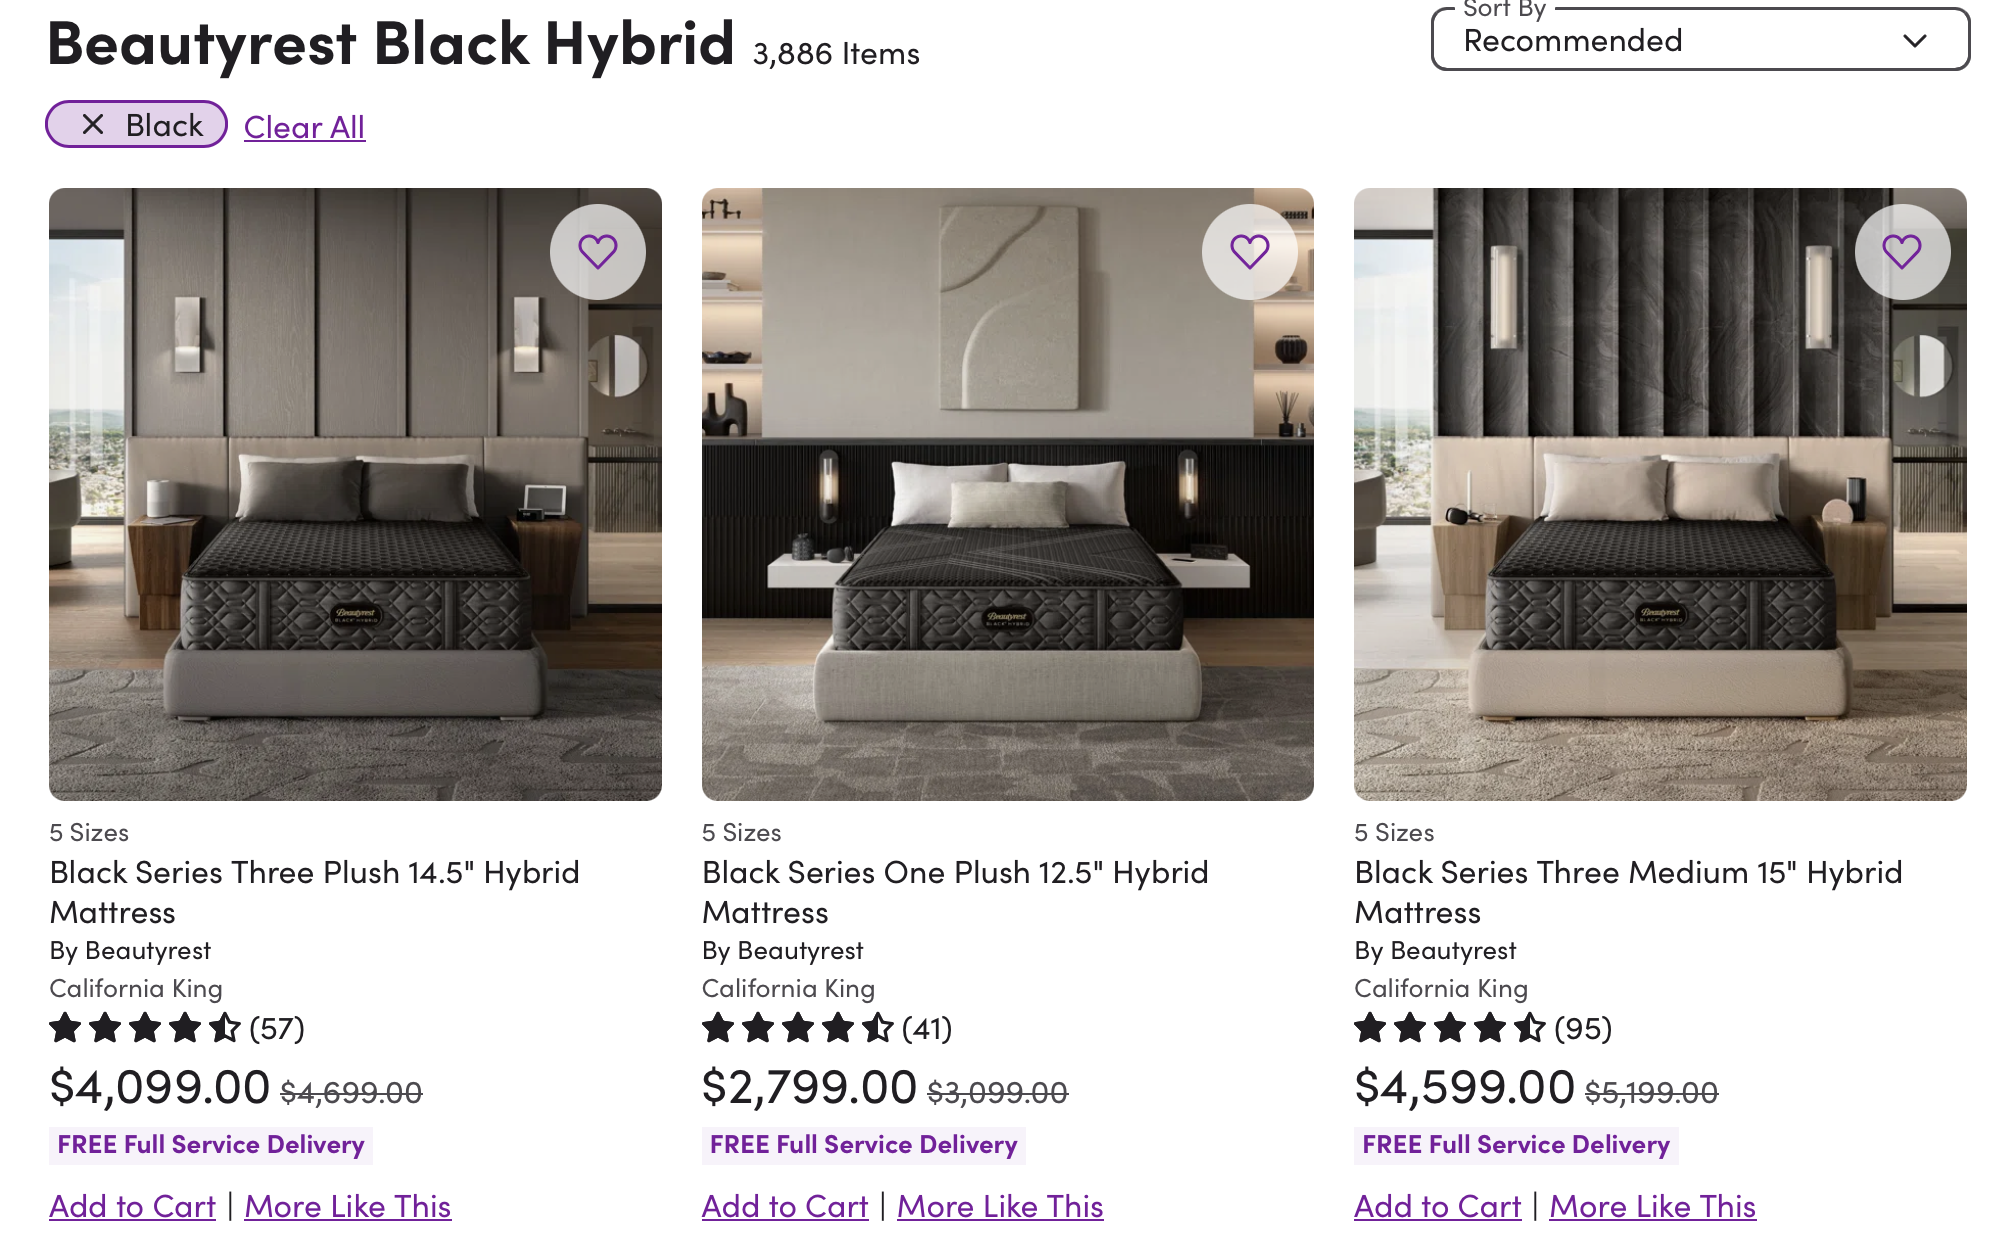
\includegraphics[width=0.9\textwidth]{figures/separate_example.png}
\end{alertblock}
\begin{itemize}
    \item 每个型号独立评分
    \item 4.4星(57评)、4.3星(41评)、4.4星(95评)
\end{itemize}

\column{0.48\textwidth}
\begin{exampleblock}{聚合展示（品牌官网）}
\centering
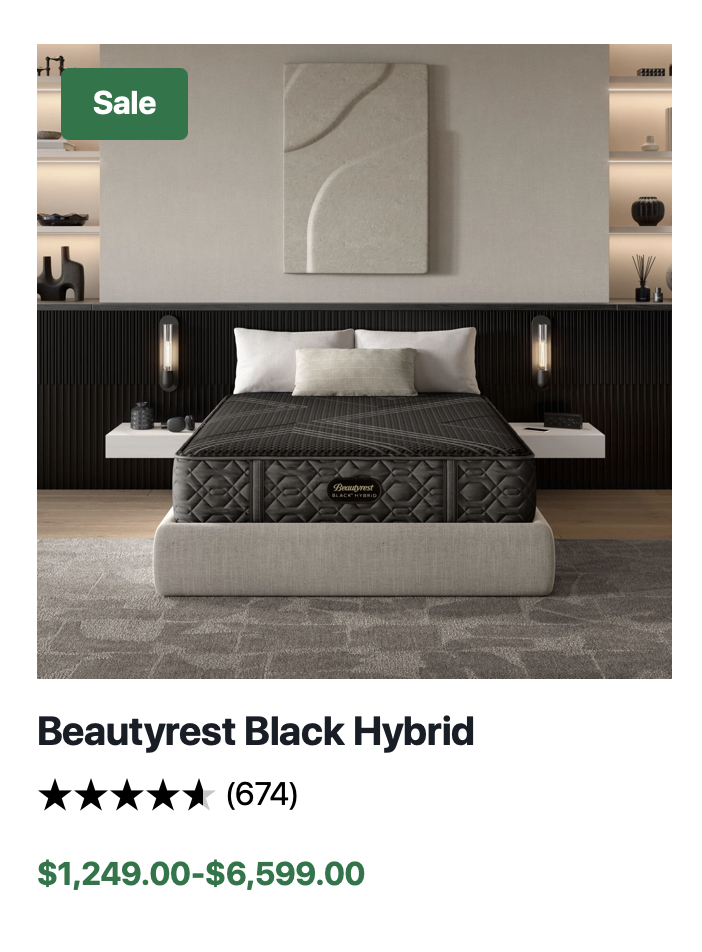
\includegraphics[width=0.45\textwidth]{figures/integrate_example.png}
\end{exampleblock}
\begin{itemize}
    \item 整个系列合并评分
    \item 4.5星(674评)
\end{itemize}
\end{columns}
\end{frame}

\begin{frame}{研究问题}
\begin{center}
\begin{tikzpicture}
    \node[draw, rounded corners, fill=positive!15, minimum width=10cm, minimum height=2cm, align=center, font=\large] {
        \textbf{核心研究问题} \\[6pt]
        对于销售\HL{垂直差异化}产品的平台，\\
        应该选择哪种评论展示策略？
    };
\end{tikzpicture}
\end{center}

\vspace{10pt}
\textbf{具体子问题}
\begin{enumerate}
    \item 两种策略下消费者的\pos{学习行为}有何不同？
    \item 策略选择如何影响平台\pos{利润}？
    \item 策略选择对\HL{消费者福利}有何影响？
    \item 评论精度非对称性如何影响策略比较？
\end{enumerate}
\end{frame}

%==============================================================================
\section{文献综述}
%==============================================================================

\begin{frame}{相关文献}
\small
\begin{center}
\begin{tabular}{p{2.8cm}p{4.2cm}p{5cm}}
\toprule
\textbf{研究领域} & \textbf{代表文献} & \textbf{与本文关系} \\
\midrule
信息设计与贝叶斯说服 & Kamenica \& Gentzkow (2011); Bergemann \& Morris (2019) & 理论框架基础 \\
\midrule
在线评论与消费者学习 & Acemoglu et al. (2022); Zhao et al. (2013) & 学习机制建模 \\
\midrule
平台评论系统设计 & Xiao et al. (2022); Shi et al. (2023) & 直接相关研究 \\
\midrule
多产品定价 & Mussa \& Rosen (1978); Johnson \& Myatt (2003) & 产品线背景 \\
\bottomrule
\end{tabular}
\end{center}

\vspace{6pt}
\textbf{本文贡献}：
\begin{itemize}
    \item 首次研究\HL{同类产品间}评论聚合与分开展示的策略选择
    \item 将信息的\pos{内生生成过程}纳入信息设计框架
    \item 引入评论精度非对称性扩展
\end{itemize}
\end{frame}

%==============================================================================
\section{模型与结果}
%==============================================================================

\subsection{模型设定}

\begin{frame}{模型概述}
\textbf{基本设定}
\begin{itemize}
    \item \textbf{参与者}：垄断平台（销售两种产品）、消费者
    \item \textbf{产品}：
    \begin{itemize}
        \item 产品B（基础版）：质量 $q_B \sim N(q_L, 1/\tau)$
        \item 产品G（高级版）：质量 $q_G \sim N(q_H, 1/\tau)$，$q_H > q_L$
    \end{itemize}
    \item \textbf{时间结构}：两期模型
\end{itemize}

\vspace{6pt}
\begin{center}
\begin{tikzpicture}[scale=0.9]
    % Timeline
    \draw[thick, ->] (0,0) -- (11,0);

    % Period markers
    \node[below] at (0,0) {$t=0$};
    \node[below] at (5,0) {$t=1$};
    \node[below] at (10,0) {$t=2$};

    % Period labels
    \node[above, align=center, font=\small] at (2.5,0.2) {第一期\\消费者购买\\评论产生};
    \node[above, align=center, font=\small] at (7.5,0.2) {第二期\\消费者学习\\更新信念};

    % Dots
    \fill (0,0) circle (2.5pt);
    \fill (5,0) circle (2.5pt);
    \fill (10,0) circle (2.5pt);
\end{tikzpicture}
\end{center}
\end{frame}

\begin{frame}{需求与评论机制}
\textbf{需求函数}
\[
k_\delta = m_\delta(v_\delta - h \cdot p_\delta), \quad \delta \in \{B, G\}
\]
其中 $v_\delta$ 为感知价值，$p_\delta$ 为价格，$h$ 为价格敏感度

\vspace{8pt}
\textbf{评论生成}
\begin{itemize}
    \item 购买者中比例 $\theta$ 发布评论
    \item 评论反映感知质量：$q_{\delta,i} \sim N(q_\delta, 1/\zeta)$
\end{itemize}

\vspace{8pt}
\textbf{评分信号}
\begin{itemize}
    \item 分开展示：$r_\delta \mid q_\delta \sim N(q_\delta, 1/(k_\delta \theta \zeta))$
    \item 聚合展示：$r_I = \frac{k_B r_B + k_G r_G}{k_B + k_G}$
\end{itemize}
\end{frame}

\begin{frame}{基本假设}
\begin{block}{假设 1：策略承诺}
平台在定价决策之前承诺评论展示策略。
\end{block}

\vspace{6pt}
\begin{block}{假设 2：评论真实性}
所有评论均为购买者的真实体验反馈，不存在虚假评论。
\end{block}

\vspace{6pt}
\begin{block}{假设 3：理性贝叶斯学习}
消费者为理性贝叶斯学习者，能够正确更新质量信念。
\end{block}
\end{frame}

\begin{frame}{平台利润函数}
\textbf{第一期利润}

由需求函数反解价格：$p_\delta = \frac{m_\delta v_\delta - k_\delta}{h \cdot m_\delta}$

第一期消费者基于先验 $v_\delta = \bar{q}_\delta$ 购买，利润为：
\[
\Pi_{\delta 1} = p_\delta \cdot k_\delta = \frac{(m_{\delta 1} \bar{q}_\delta - k_\delta) \cdot k_\delta}{h \cdot m_{\delta 1}}
\]

\vspace{6pt}
\textbf{第二期最优定价}

给定后验感知价值 $v_\delta$，平台最大化 $\Pi_{\delta 2} = p \cdot m_{\delta 2}(v_\delta - hp)$

一阶条件得最优价格：$p^*_{\delta 2} = \frac{v_\delta}{2h}$，最优利润：
\[
\Pi^*_{\delta 2} = \frac{m_{\delta 2} \cdot \max\{0, v_\delta\}^2}{4h}
\]

\vspace{6pt}
\textbf{总利润}：$\Pi = \sum_{\delta \in \{B,G\}} (\Pi_{\delta 1} + \E[\Pi^*_{\delta 2}])$
\end{frame}

\begin{frame}{利润与后验方差的关系}
\textbf{关键洞察}

第二期期望利润：
\[
\E[\Pi^*_{\delta 2}] = \frac{m_{\delta 2}}{4h} \cdot \E[\max\{0, v_\delta\}^2]
\]

由于 $v_\delta \sim N(\bar{q}_\delta, \sigma^2_\delta)$ 且 $\bar{q}_\delta > 0$：

\vspace{6pt}
\begin{block}{引理：期望利润关于方差递增}
对于均值 $\mu > 0$ 的正态随机变量 $v \sim N(\mu, \sigma^2)$，
\[
\frac{\partial}{\partial \sigma^2} \E[\max\{0, v\}^2] > 0
\]
\end{block}

\vspace{6pt}
\textbf{经济含义}：
\begin{itemize}
    \item 后验方差 $\sigma^2_\delta$ 越大 $\Rightarrow$ 评分对信念影响越大 $\Rightarrow$ 信息越有价值
    \item 平台可根据已揭示的质量信息调整价格（\HL{状态依存定价}）
    \item 如果分开展示 $\sigma^2_S > \sigma^2_I$ $\Rightarrow$ \pos{分开展示利润更高}
\end{itemize}
\end{frame}

\subsection{分开展示分析}

\begin{frame}{分开展示：贝叶斯更新}
\textbf{后验分布}（命题 4.1）

消费者观察独立评分 $r_\delta$，后验信念：
\[
q_\delta \mid r_\delta \sim N\left(\frac{\tau \bar{q}_\delta + k_\delta\theta\zeta \cdot r_\delta}{\tau + k_\delta\theta\zeta}, \frac{1}{\tau + k_\delta\theta\zeta}\right)
\]

\vspace{8pt}
\textbf{后验均值的先验分布}（引理 4.1）
\begin{align*}
\E[v_{S\delta}] &= \bar{q}_\delta \\[4pt]
\Var[v_{S\delta}] &= \sigma_{S\delta}^2 = \frac{k_\delta\theta\zeta}{\tau^2 + k_\delta\tau\theta\zeta}
\end{align*}

\vspace{6pt}
\HL{关键特征}：两种产品的定价决策\textbf{相互独立}
\end{frame}

\subsection{聚合展示分析}

\begin{frame}{聚合展示：贝叶斯更新}
\textbf{后验分布}（命题 5.1）

消费者仅观察综合评分 $r_I$，需对另一产品质量积分：
\[
v_{IB} = \frac{(k_B + k_G)k_B\theta\zeta \cdot r_I - k_B k_G\theta\zeta \cdot q_H + [k_G^2\theta\zeta + (k_B + k_G)\tau] \cdot q_L}{(k_B^2 + k_G^2)\theta\zeta + (k_B + k_G)\tau}
\]

\vspace{8pt}
\textbf{后验均值的先验分布}（引理 5.1）
\begin{align*}
\E[v_{I\delta}] &= \bar{q}_\delta \\[4pt]
\Var[v_{I\delta}] &= \sigma_{I\delta}^2 = \frac{k_\delta^2\theta\zeta}{(k_B^2 + k_G^2)\tau\theta\zeta + (k_B + k_G)\tau^2}
\end{align*}

\vspace{6pt}
\con{关键特征}：两种产品的定价决策\textbf{相互耦合}
\end{frame}

\begin{frame}{聚合展示降低信息精度}
\begin{block}{命题 5.2：信息稀释效应}
对于任意给定的购买量 $(k_B, k_G)$，聚合展示下消费者信念的方差\textbf{不超过}分开展示：
\[
\sigma_{I\delta}^2 \leq \sigma_{S\delta}^2, \quad \delta \in \{B, G\}
\]
等号当且仅当 $k_B = 0$ 或 $k_G = 0$ 时成立。
\end{block}

\vspace{8pt}
\textbf{经济含义}：
\begin{itemize}
    \item 聚合展示混合不同质量产品的评论
    \item 引入\con{评论来源不确定性}
    \item 消费者无法区分评分中的信息来源
    \item 后验方差更低 $\Rightarrow$ 评分对信念影响更小 $\Rightarrow$ \con{学习效率降低}
\end{itemize}
\end{frame}

\subsection{策略比较}

\begin{frame}{核心结果一：给定购买量下分开展示占优}
\begin{block}{命题 5.3}
对于任意给定的 $(k_B, k_G)$ 且 $k_B > 0$, $k_G > 0$，分开展示的期望总利润\textbf{严格高于}聚合展示：
\[
\E[\Pi_S \mid k_B, k_G] > \E[\Pi_I \mid k_B, k_G]
\]
\end{block}

\vspace{8pt}
\textbf{证明思路}：
\begin{itemize}
    \item 第一期利润相同（给定相同购买量）
    \item 第二期利润差异来自后验方差
    \item 对于均值 $\mu > 0$ 的正态变量，$\E[\max\{0, v^2\}]$ 关于方差严格递增
    \item 分开展示方差更大 $\Rightarrow$ 第二期利润更高
\end{itemize}
\end{frame}

\begin{frame}{核心结果二：两倍信息效率}
\begin{block}{命题 5.4：分开展示的信息效率优势}
在对称情形下（$k_B = k_G = k$），分开展示对第二期利润的期望贡献恰好是聚合展示的\textbf{两倍}：
\[
\frac{m\sigma_{SB}^2 + m\sigma_{SG}^2}{m\sigma_{IB}^2 + m\sigma_{IG}^2} = 2
\]
\end{block}

\vspace{8pt}
\textbf{经济解释}：
\begin{itemize}
    \item 聚合展示将样本量从 $k$ 增加到 $2k$
    \item 但\con{来源不确定性}抵消了样本规模收益
    \item 净效果：有效信息量\con{减半}
    \item 该 2:1 比例与质量差距 $\Delta q$ \textbf{无关}
\end{itemize}
\end{frame}

\begin{frame}{核心结果三：分开展示普遍占优}
\begin{block}{命题 5.5：分开展示的普遍优势（数值验证）}
在本文模型设定下，对于\textbf{所有测试的参数配置}，分开展示策略在最优决策下均产生严格更高的期望利润：
\[
\Pi_S^*(k_{SB}^*, k_{SG}^*) > \Pi_I^*(k_{IB}^*, k_{IG}^*)
\]
\end{block}

\vspace{8pt}
\textbf{为什么聚合展示无法逆转劣势？}
\begin{enumerate}
    \item \pos{信息价值为正}：精确信号 $\Rightarrow$ 状态依存定价 $\Rightarrow$ 期望收益增加
    \item \con{样本规模优势不足}：来源不确定性成本 $>$ 样本合并收益
    \item \con{交叉效应有限}：最优购买量差异仅 5--7\%，不足以改变排序
\end{enumerate}
\end{frame}

%==============================================================================
\section{数值分析与扩展}
%==============================================================================

\subsection{数值模拟}

\begin{frame}{数值模拟设定}
\textbf{基准参数}

\vspace{4pt}
\begin{center}
\small
\begin{tabular}{ccc}
\toprule
\textbf{参数} & \textbf{符号} & \textbf{基准值} \\
\midrule
低质量产品均值 & $q_L$ & 1.0 \\
高质量产品均值 & $q_H$ & 2.0 \\
先验精度 & $\tau$ & 1.0 \\
感知精度 & $\zeta$ & 1.0 \\
评论生成概率 & $\theta$ & 0.5 \\
价格敏感度 & $h$ & 1.0 \\
市场规模 & $m_{\delta t}$ & 1.0 \\
\bottomrule
\end{tabular}
\end{center}

\vspace{6pt}
\textbf{基准结果}：$\Pi_S^* = 2.6355$，$\Pi_I^* = 2.5741$，利润差 $= 0.0613$
\end{frame}

\begin{frame}{敏感性分析}
\begin{columns}[T]
\column{0.55\textwidth}
\begin{center}
\begin{tikzpicture}[scale=0.8]
\begin{axis}[
    xlabel={参数值},
    ylabel={利润差 $\Pi_S^* - \Pi_I^*$},
    legend pos=outer north east,
    legend style={font=\footnotesize},
    grid=major,
    width=7.5cm, height=5.5cm,
    xmin=0, xmax=2.5,
    ymin=0, ymax=1.5
]
    \addplot[thick, positive, domain=0.1:2.5, samples=30] {0.055 + 0.003*x};
    \addlegendentry{$\Delta q$}

    \addplot[thick, negative, dashed, domain=0.1:2.5, samples=30] {1.5*exp(-1.5*x) + 0.02};
    \addlegendentry{$\tau$}

    \addplot[thick, emphasis, dotted, domain=0.1:2.5, samples=30] {0.1*x};
    \addlegendentry{$\theta$}

    \draw[dashed, gray] (axis cs:0,0) -- (axis cs:2.5,0);
\end{axis}
\end{tikzpicture}
\end{center}

\column{0.42\textwidth}
\textbf{关键发现}

\vspace{6pt}
\begin{itemize}
    \item 利润差 $\Pi_S^* - \Pi_I^*$ \textbf{始终为正}

    \vspace{4pt}
    \item \pos{先验精度 $\tau$} 影响最显著：
    \begin{itemize}
        \item $\tau$ 低（不确定性高）$\Rightarrow$ 分开展示优势大
    \end{itemize}

    \vspace{4pt}
    \item 质量差距 $\Delta q$ 影响有限

    \vspace{4pt}
    \item 评论率 $\theta$ 越高，优势越明显
\end{itemize}
\end{columns}
\end{frame}

\subsection{福利分析}

\begin{frame}{福利分析：利润与福利目标一致}
\textbf{消费者剩余}
\[
CS_{\psi 2} = \frac{m_{B2} \cdot \E[\max\{0, v_{\psi B}^2\}]}{8h} + \frac{m_{G2} \cdot \E[\max\{0, v_{\psi G}^2\}]}{8h}
\]

\vspace{6pt}
\begin{block}{命题 5.6：分开展示的福利优势}
在本文模型设定下，分开展示策略\textbf{同时}最大化平台利润、消费者剩余和社会总福利：
\[
\Pi_S^* > \Pi_I^*, \quad CS_S^* > CS_I^*, \quad W_S^* > W_I^*
\]
\end{block}

\vspace{6pt}
\textbf{重要结论}：
\begin{itemize}
    \item 平台利润最大化与社会福利最大化\HL{指向同一策略}
    \item \pos{不存在利润-福利冲突}
    \item 与信息设计文献中常见的权衡不同
\end{itemize}
\end{frame}

\subsection{模型扩展}

\begin{frame}{扩展：评论精度非对称性}
\textbf{扩展动机}
\begin{itemize}
    \item 高质量产品用户评论可能更详细、更精确
    \item 不同产品的用户群体评论质量可能不同
\end{itemize}

\vspace{6pt}
\textbf{扩展设定}：$\zeta_B \neq \zeta_G$，定义精度比 $\rho = \zeta_G / \zeta_B$

\vspace{6pt}
\begin{block}{命题 6.1：精度非对称性放大分开展示优势}
定义信息效率比 $\mathcal{R}(\rho) = \frac{m\sigma_{SB}^2 + m\sigma_{SG}^2}{m\sigma_{IB}^2 + m\sigma_{IG}^2}$，则：
\begin{itemize}
    \item 当 $\rho = 1$（对称）时，$\mathcal{R}(1) = 2$
    \item 当 $\rho \neq 1$ 时，$\mathcal{R}(\rho) > 2$
\end{itemize}
\end{block}
\end{frame}

\begin{frame}{扩展：数值验证}
\begin{center}
\small
\begin{tabular}{ccccc}
\toprule
$\rho = \zeta_G/\zeta_B$ & 分开展示利润 & 聚合展示利润 & 利润差 & 信息比 $\mathcal{R}$ \\
\midrule
0.25 & 2.4821 & 2.3056 & 0.1765 & 2.89 \\
0.50 & 2.5634 & 2.4412 & 0.1222 & 2.41 \\
1.00 & 2.6355 & 2.5741 & 0.0613 & 2.00 \\
2.00 & 2.7089 & 2.5623 & 0.1466 & 2.48 \\
4.00 & 2.7845 & 2.4987 & 0.2858 & 3.12 \\
\bottomrule
\end{tabular}
\end{center}

\vspace{8pt}
\begin{block}{命题 6.2：基准结论的稳健性}
"分开展示普遍占优"的结论对评论精度的非对称性具有稳健性。精度非对称性是分开展示优势的\HL{放大因素}而非逆转因素。
\end{block}
\end{frame}

%==============================================================================
\section{结论与展望}
%==============================================================================

\begin{frame}{主要结论}
\begin{enumerate}
    \item \textbf{聚合展示降低信息精度}
    \begin{itemize}
        \item 引入"评论来源不确定性"，消费者学习效率降低
    \end{itemize}

    \vspace{6pt}
    \item \textbf{分开展示普遍占优}
    \begin{itemize}
        \item 对称情形下信息效率 2:1
        \item 所有测试参数下均占优
    \end{itemize}

    \vspace{6pt}
    \item \textbf{利润与福利目标一致}
    \begin{itemize}
        \item 分开展示同时最大化利润、消费者剩余和社会福利
        \item 不存在利润-福利冲突
    \end{itemize}

    \vspace{6pt}
    \item \textbf{评论精度非对称性强化结论}
    \begin{itemize}
        \item 精度差异越大，分开展示优势越明显
    \end{itemize}
\end{enumerate}
\end{frame}

\begin{frame}{管理启示与未来方向}
\textbf{管理启示}
\begin{itemize}
    \item 垂直差异化产品组合：优先采用\pos{分开展示}
    \item 高质量评论是信息资产，避免与低质量评论混合稀释
    \item 可通过评论标签、评论者等级提升评论精度差异化
\end{itemize}

\vspace{10pt}
\textbf{未来研究方向}
\begin{itemize}
    \item \textbf{模型拓展}：多产品（$>2$）、动态评论积累、竞争平台
    \item \textbf{机制拓展}：消费者异质性学习、评论操纵成本
    \item \textbf{实证研究}：利用平台数据检验理论预测
\end{itemize}
\end{frame}

%==============================================================================
\section*{参考文献}
%==============================================================================

\begin{frame}{参考文献}
\small
\begin{thebibliography}{9}
\bibitem{kamenica2011} Kamenica, E., \& Gentzkow, M. (2011). Bayesian persuasion. \textit{American Economic Review}, 101(6), 2590--2615.

\bibitem{acemoglu2022} Acemoglu, D., et al. (2022). Learning from reviews: The selection effect and the speed of learning. \textit{Econometrica}, 90(6), 2857--2899.

\bibitem{xiao2022} Xiao, P., Chen, Z., \& Tang, C. S. (2022). Customer review provision policies in e-commerce. \textit{Production and Operations Management}, 31(12), 4429--4443.

\bibitem{shi2023} Shi, Z., Srinivasan, K., \& Zhang, K. (2023). Design of platform reputation systems. \textit{Marketing Science}, 42(2), 310--331.

\bibitem{bergemann2019} Bergemann, D., \& Morris, S. (2019). Information design: A unified perspective. \textit{Journal of Economic Literature}, 57(1), 44--95.
\end{thebibliography}
\end{frame}

%==============================================================================
% 致谢
%==============================================================================

\begin{frame}
\begin{center}
\vspace{1.5cm}
{\Huge 谢谢！}

\vspace{0.8cm}
{\large 欢迎提问与讨论}

\vspace{1.2cm}
{\small 联系方式：jiaoyang2022@shanghaitech.edu.cn}
\end{center}
\end{frame}

%==============================================================================
\appendix
%==============================================================================

\begin{frame}{备用幻灯片}
\begin{center}
\textit{以下为备用幻灯片，用于Q\&A环节}
\end{center}
\end{frame}

\begin{frame}{符号汇总}
\begin{center}
\small
\begin{tabular}{cll}
\toprule
\textbf{符号} & \textbf{含义} & \textbf{基准值} \\
\midrule
$q_L, q_H$ & 产品质量先验均值 & 1.0, 2.0 \\
$\tau$ & 质量先验精度 & 1.0 \\
$\zeta$ & 评论感知精度 & 1.0 \\
$\theta$ & 评论生成概率 & 0.5 \\
$k_\delta$ & 产品 $\delta$ 第一期购买量 & (内生) \\
$m_{\delta t}$ & 产品 $\delta$ 在 $t$ 期的市场规模 & 1.0 \\
$h$ & 价格敏感度 & 1.0 \\
$\sigma_{S\delta}^2, \sigma_{I\delta}^2$ & 后验方差（分开/聚合） & (内生) \\
$\rho$ & 评论精度比 $\zeta_G/\zeta_B$ & 1.0 \\
\bottomrule
\end{tabular}
\end{center}
\end{frame}

\begin{frame}{贝叶斯更新推导细节}
\textbf{分开展示下的后验}

给定 $n = k_\delta \theta$ 个评论信号，后验分布为：
\[
q_\delta \mid \{r_i\} \sim N\left(\frac{\tau \bar{q}_\delta + n\zeta\bar{r}}{\tau + n\zeta}, \frac{1}{\tau + n\zeta}\right)
\]

\vspace{6pt}
\textbf{后验均值的方差推导}

由于 $\bar{r} = q_\delta + \bar{\epsilon}$，后验均值 $\hat{q}_\delta$ 的方差为：
\[
\Var(\hat{q}_\delta) = \left(\frac{n\zeta}{\tau + n\zeta}\right)^2 \cdot \frac{1}{n\zeta} = \frac{n\zeta}{(\tau + n\zeta)^2}
\]

代入 $n = k_\delta \theta$ 并整理：
\[
\sigma_{S\delta}^2 = \frac{k_\delta\theta\zeta}{\tau^2 + k_\delta\tau\theta\zeta}
\]
\end{frame}

\begin{frame}{聚合展示可能占优的扩展方向}
\textbf{本文基准模型下分开展示普遍占优，但以下扩展可能改变结论：}

\vspace{6pt}
\begin{enumerate}
    \item \textbf{消费者异质性学习能力}
    \begin{itemize}
        \item "朴素型"消费者偏好评论数量 $\Rightarrow$ 聚合展示可能占优
    \end{itemize}

    \vspace{4pt}
    \item \textbf{评论操纵与信誉成本}
    \begin{itemize}
        \item 分开展示使负面信号更可见 $\Rightarrow$ 信誉成本高时聚合可能占优
    \end{itemize}

    \vspace{4pt}
    \item \textbf{多期动态与产品多样性}
    \begin{itemize}
        \item 聚合展示可保护弱势产品 $\Rightarrow$ 长期多样性价值高时可能占优
    \end{itemize}

    \vspace{4pt}
    \item \textbf{竞争性平台}
    \begin{itemize}
        \item 展示策略可作为差异化工具 $\Rightarrow$ 可能存在非对称均衡
    \end{itemize}
\end{enumerate}
\end{frame}

\end{document}
